% Options for packages loaded elsewhere
\PassOptionsToPackage{unicode}{hyperref}
\PassOptionsToPackage{hyphens}{url}
%
\documentclass[
]{book}
\usepackage{lmodern}
\usepackage{amssymb,amsmath}
\usepackage{ifxetex,ifluatex}
\ifnum 0\ifxetex 1\fi\ifluatex 1\fi=0 % if pdftex
  \usepackage[T1]{fontenc}
  \usepackage[utf8]{inputenc}
  \usepackage{textcomp} % provide euro and other symbols
\else % if luatex or xetex
  \usepackage{unicode-math}
  \defaultfontfeatures{Scale=MatchLowercase}
  \defaultfontfeatures[\rmfamily]{Ligatures=TeX,Scale=1}
\fi
% Use upquote if available, for straight quotes in verbatim environments
\IfFileExists{upquote.sty}{\usepackage{upquote}}{}
\IfFileExists{microtype.sty}{% use microtype if available
  \usepackage[]{microtype}
  \UseMicrotypeSet[protrusion]{basicmath} % disable protrusion for tt fonts
}{}
\makeatletter
\@ifundefined{KOMAClassName}{% if non-KOMA class
  \IfFileExists{parskip.sty}{%
    \usepackage{parskip}
  }{% else
    \setlength{\parindent}{0pt}
    \setlength{\parskip}{6pt plus 2pt minus 1pt}}
}{% if KOMA class
  \KOMAoptions{parskip=half}}
\makeatother
\usepackage{xcolor}
\IfFileExists{xurl.sty}{\usepackage{xurl}}{} % add URL line breaks if available
\IfFileExists{bookmark.sty}{\usepackage{bookmark}}{\usepackage{hyperref}}
\hypersetup{
  pdftitle={Plotting in R using ggplot},
  pdfauthor={Vratika Chaudhary},
  hidelinks,
  pdfcreator={LaTeX via pandoc}}
\urlstyle{same} % disable monospaced font for URLs
\usepackage{color}
\usepackage{fancyvrb}
\newcommand{\VerbBar}{|}
\newcommand{\VERB}{\Verb[commandchars=\\\{\}]}
\DefineVerbatimEnvironment{Highlighting}{Verbatim}{commandchars=\\\{\}}
% Add ',fontsize=\small' for more characters per line
\usepackage{framed}
\definecolor{shadecolor}{RGB}{248,248,248}
\newenvironment{Shaded}{\begin{snugshade}}{\end{snugshade}}
\newcommand{\AlertTok}[1]{\textcolor[rgb]{0.94,0.16,0.16}{#1}}
\newcommand{\AnnotationTok}[1]{\textcolor[rgb]{0.56,0.35,0.01}{\textbf{\textit{#1}}}}
\newcommand{\AttributeTok}[1]{\textcolor[rgb]{0.77,0.63,0.00}{#1}}
\newcommand{\BaseNTok}[1]{\textcolor[rgb]{0.00,0.00,0.81}{#1}}
\newcommand{\BuiltInTok}[1]{#1}
\newcommand{\CharTok}[1]{\textcolor[rgb]{0.31,0.60,0.02}{#1}}
\newcommand{\CommentTok}[1]{\textcolor[rgb]{0.56,0.35,0.01}{\textit{#1}}}
\newcommand{\CommentVarTok}[1]{\textcolor[rgb]{0.56,0.35,0.01}{\textbf{\textit{#1}}}}
\newcommand{\ConstantTok}[1]{\textcolor[rgb]{0.00,0.00,0.00}{#1}}
\newcommand{\ControlFlowTok}[1]{\textcolor[rgb]{0.13,0.29,0.53}{\textbf{#1}}}
\newcommand{\DataTypeTok}[1]{\textcolor[rgb]{0.13,0.29,0.53}{#1}}
\newcommand{\DecValTok}[1]{\textcolor[rgb]{0.00,0.00,0.81}{#1}}
\newcommand{\DocumentationTok}[1]{\textcolor[rgb]{0.56,0.35,0.01}{\textbf{\textit{#1}}}}
\newcommand{\ErrorTok}[1]{\textcolor[rgb]{0.64,0.00,0.00}{\textbf{#1}}}
\newcommand{\ExtensionTok}[1]{#1}
\newcommand{\FloatTok}[1]{\textcolor[rgb]{0.00,0.00,0.81}{#1}}
\newcommand{\FunctionTok}[1]{\textcolor[rgb]{0.00,0.00,0.00}{#1}}
\newcommand{\ImportTok}[1]{#1}
\newcommand{\InformationTok}[1]{\textcolor[rgb]{0.56,0.35,0.01}{\textbf{\textit{#1}}}}
\newcommand{\KeywordTok}[1]{\textcolor[rgb]{0.13,0.29,0.53}{\textbf{#1}}}
\newcommand{\NormalTok}[1]{#1}
\newcommand{\OperatorTok}[1]{\textcolor[rgb]{0.81,0.36,0.00}{\textbf{#1}}}
\newcommand{\OtherTok}[1]{\textcolor[rgb]{0.56,0.35,0.01}{#1}}
\newcommand{\PreprocessorTok}[1]{\textcolor[rgb]{0.56,0.35,0.01}{\textit{#1}}}
\newcommand{\RegionMarkerTok}[1]{#1}
\newcommand{\SpecialCharTok}[1]{\textcolor[rgb]{0.00,0.00,0.00}{#1}}
\newcommand{\SpecialStringTok}[1]{\textcolor[rgb]{0.31,0.60,0.02}{#1}}
\newcommand{\StringTok}[1]{\textcolor[rgb]{0.31,0.60,0.02}{#1}}
\newcommand{\VariableTok}[1]{\textcolor[rgb]{0.00,0.00,0.00}{#1}}
\newcommand{\VerbatimStringTok}[1]{\textcolor[rgb]{0.31,0.60,0.02}{#1}}
\newcommand{\WarningTok}[1]{\textcolor[rgb]{0.56,0.35,0.01}{\textbf{\textit{#1}}}}
\usepackage{longtable,booktabs}
% Correct order of tables after \paragraph or \subparagraph
\usepackage{etoolbox}
\makeatletter
\patchcmd\longtable{\par}{\if@noskipsec\mbox{}\fi\par}{}{}
\makeatother
% Allow footnotes in longtable head/foot
\IfFileExists{footnotehyper.sty}{\usepackage{footnotehyper}}{\usepackage{footnote}}
\makesavenoteenv{longtable}
\usepackage{graphicx,grffile}
\makeatletter
\def\maxwidth{\ifdim\Gin@nat@width>\linewidth\linewidth\else\Gin@nat@width\fi}
\def\maxheight{\ifdim\Gin@nat@height>\textheight\textheight\else\Gin@nat@height\fi}
\makeatother
% Scale images if necessary, so that they will not overflow the page
% margins by default, and it is still possible to overwrite the defaults
% using explicit options in \includegraphics[width, height, ...]{}
\setkeys{Gin}{width=\maxwidth,height=\maxheight,keepaspectratio}
% Set default figure placement to htbp
\makeatletter
\def\fps@figure{htbp}
\makeatother
\setlength{\emergencystretch}{3em} % prevent overfull lines
\providecommand{\tightlist}{%
  \setlength{\itemsep}{0pt}\setlength{\parskip}{0pt}}
\setcounter{secnumdepth}{5}
\usepackage{booktabs}
\usepackage[]{natbib}
\bibliographystyle{apalike}

\title{Plotting in R using ggplot}
\author{Vratika Chaudhary}
\date{2020-12-10}

\begin{document}
\maketitle

{
\setcounter{tocdepth}{1}
\tableofcontents
}
\hypertarget{prerequisites}{%
\chapter{Prerequisites}\label{prerequisites}}

R programming language
Installed packages:

\begin{Shaded}
\begin{Highlighting}[]
\NormalTok{pkg<-}\KeywordTok{c}\NormalTok{(}\StringTok{"ggplot2"}\NormalTok{,}\StringTok{"ggpubr"}\NormalTok{,}\StringTok{"auk"}\NormalTok{,}\StringTok{"datasets"}\NormalTok{,}\StringTok{"ggpubr"}\NormalTok{,}\StringTok{"ggcorrplot"}\NormalTok{)}
\KeywordTok{install.packages}\NormalTok{(pkg)}
\end{Highlighting}
\end{Shaded}

\hypertarget{intro}{%
\chapter{Data preperation}\label{intro}}

We can enter CSV data in R using read.csv function or read\_csv function from readr package. However, for now we will use data that already exist in the datasets packages that we downloaded

Lets load the library `datsets'

\begin{Shaded}
\begin{Highlighting}[]
\KeywordTok{library}\NormalTok{(datasets)}
\end{Highlighting}
\end{Shaded}

Lets look at the chickeweight data

\begin{Shaded}
\begin{Highlighting}[]
\KeywordTok{head}\NormalTok{(ChickWeight)}
\end{Highlighting}
\end{Shaded}

\begin{verbatim}
##   weight Time Chick Diet
## 1     42    0     1    1
## 2     51    2     1    1
## 3     59    4     1    1
## 4     64    6     1    1
## 5     76    8     1    1
## 6     93   10     1    1
\end{verbatim}

\hypertarget{introduction-to-ggplot2}{%
\chapter{Introduction to ggplot2}\label{introduction-to-ggplot2}}

The package ggplot2 is extremely functional and useful. It created graphs in layers and therefore is very intutive. It adds layers on top of each other

\hypertarget{creating-the-building-blocks-of-the-graph}{%
\section{Creating the building blocks of the graph}\label{creating-the-building-blocks-of-the-graph}}

ggplot(data = dataname, mapping= aes(x=xaxis, y= yaxis))

ggplot function from ggplot2 package requires two arguments:
data is the object name you gave to your data sets
Mapping is the specifications of the variables we want to visualize and are places withing the `aes' function short for aesthetics.

Let's bring back the chick data and let's look how chicks have grown over time

\begin{Shaded}
\begin{Highlighting}[]
\KeywordTok{library}\NormalTok{(ggplot2)}
\KeywordTok{par}\NormalTok{(}\DataTypeTok{mar =} \KeywordTok{c}\NormalTok{(}\DecValTok{4}\NormalTok{, }\DecValTok{4}\NormalTok{, }\FloatTok{.1}\NormalTok{, }\FloatTok{.1}\NormalTok{))}
\KeywordTok{ggplot}\NormalTok{(}\DataTypeTok{data=}\NormalTok{ChickWeight, }\DataTypeTok{mapping=}\KeywordTok{aes}\NormalTok{(}\DataTypeTok{x=}\NormalTok{Time, }\DataTypeTok{y=}\NormalTok{weight))}
\end{Highlighting}
\end{Shaded}

\begin{figure}

{\centering 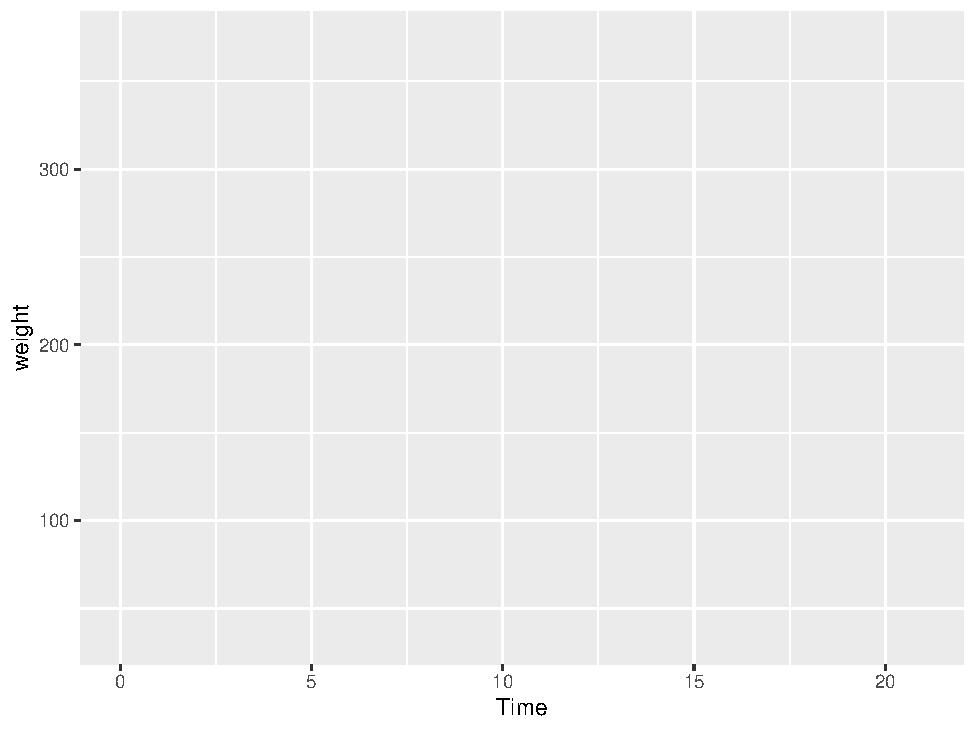
\includegraphics[width=0.8\linewidth]{plotting_r_files/figure-latex/nice-fig-1} 

}

\caption{Building block}\label{fig:nice-fig}
\end{figure}

We see a box, and we see the correct axis but we don't see anything else- why?

\hypertarget{adding-geom_objects}{%
\section{Adding geom\_objects}\label{adding-geom_objects}}

Because yes we told ggplot what variables we want to plot, but we haven't told it what type of plot we want.
We can do this by adding a `geom\_object'. For this purpose, let's make a line plot. We can do so by adding a `geom\_line' object to the previous layer. We join the two layers by a `+' sign.

\begin{Shaded}
\begin{Highlighting}[]
\KeywordTok{library}\NormalTok{(ggplot2)}

\KeywordTok{ggplot}\NormalTok{(ChickWeight, }\DataTypeTok{mapping=} \KeywordTok{aes}\NormalTok{(}\DataTypeTok{x=}\NormalTok{Time, }\DataTypeTok{y=}\NormalTok{weight))}\OperatorTok{+}
\StringTok{  }\KeywordTok{geom_line}\NormalTok{()}
\end{Highlighting}
\end{Shaded}

\begin{figure}

{\centering 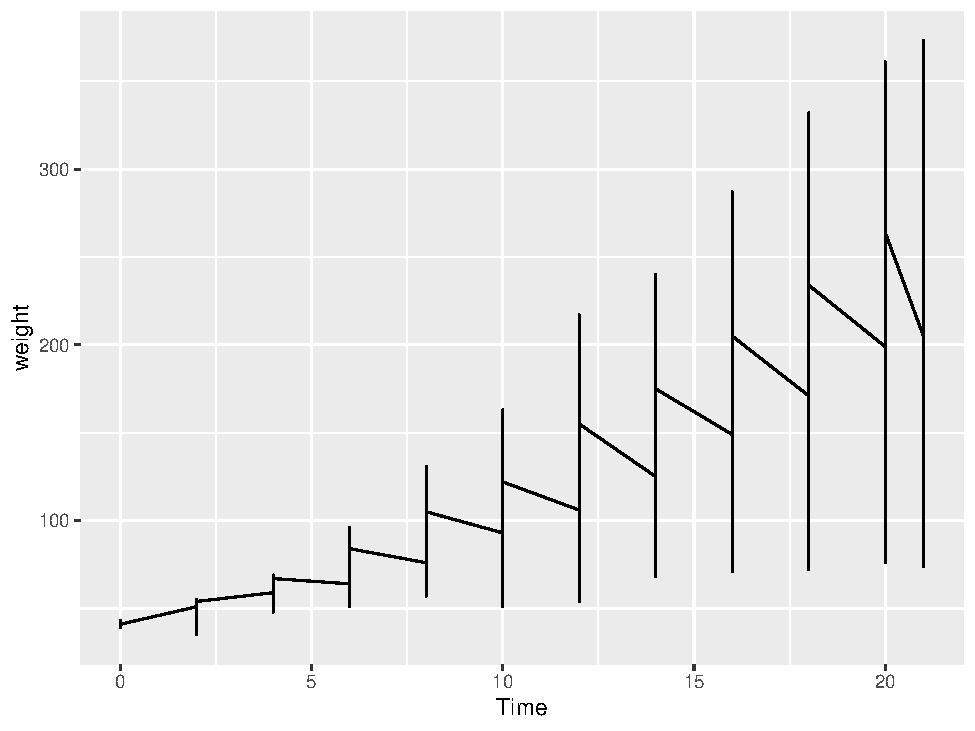
\includegraphics[width=0.8\linewidth]{plotting_r_files/figure-latex/unnamed-chunk-5-1} 

}

\caption{Line plot}\label{fig:unnamed-chunk-5}
\end{figure}

Hey! We got some lines, but it looks weird!!!
That is becasue we plotted all the data together, we had 48 chicks but we plotted all of them in the same plot. So let's make them distinct. We can simply do so by giving a distinct line to each chick by adding group

\begin{Shaded}
\begin{Highlighting}[]
\KeywordTok{library}\NormalTok{(ggplot2)}

\KeywordTok{ggplot}\NormalTok{(ChickWeight, }\KeywordTok{aes}\NormalTok{(}\DataTypeTok{x=}\NormalTok{Time, }\DataTypeTok{y=}\NormalTok{weight, }\DataTypeTok{group=}\NormalTok{Chick))}\OperatorTok{+}
\StringTok{  }\KeywordTok{geom_line}\NormalTok{()}
\end{Highlighting}
\end{Shaded}

\begin{figure}

{\centering 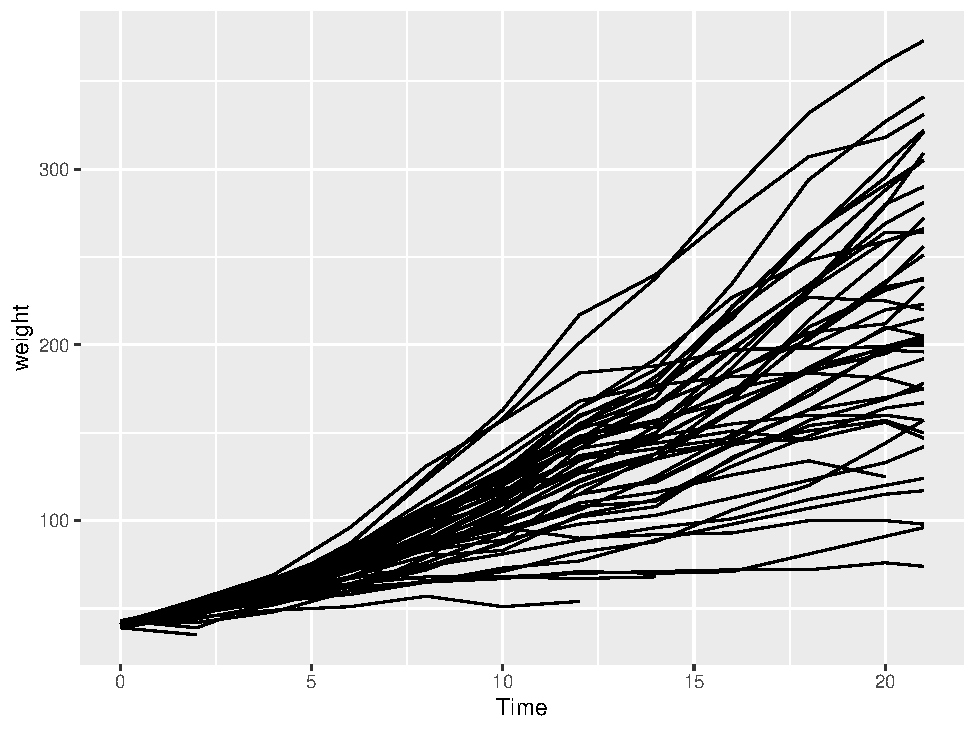
\includegraphics[width=0.8\linewidth]{plotting_r_files/figure-latex/unnamed-chunk-6-1} 

}

\caption{Line plot with colors}\label{fig:unnamed-chunk-6}
\end{figure}

\hypertarget{making-the-plot-visually-more-appealing}{%
\section{Making the plot visually more appealing}\label{making-the-plot-visually-more-appealing}}

Let's do the following:
1. Increase the size of the lines
2. Lighten the background using the theme function in ggplot2
3. Increase the size of axis text and titles
4. Change y axis label

\begin{Shaded}
\begin{Highlighting}[]
\KeywordTok{library}\NormalTok{(ggplot2)}

\KeywordTok{ggplot}\NormalTok{(ChickWeight, }\KeywordTok{aes}\NormalTok{(}\DataTypeTok{x=}\NormalTok{Time, }\DataTypeTok{y=}\NormalTok{weight, }\DataTypeTok{group=}\NormalTok{Chick),}\DataTypeTok{size=}\DecValTok{2}\NormalTok{)}\OperatorTok{+}
\StringTok{  }\KeywordTok{geom_line}\NormalTok{()}\OperatorTok{+}
\StringTok{  }\KeywordTok{theme_minimal}\NormalTok{(}\DataTypeTok{base_size =} \DecValTok{20}\NormalTok{)}\OperatorTok{+}
\StringTok{  }\KeywordTok{ylab}\NormalTok{(}\StringTok{"Weight"}\NormalTok{)}
\end{Highlighting}
\end{Shaded}

\begin{figure}

{\centering 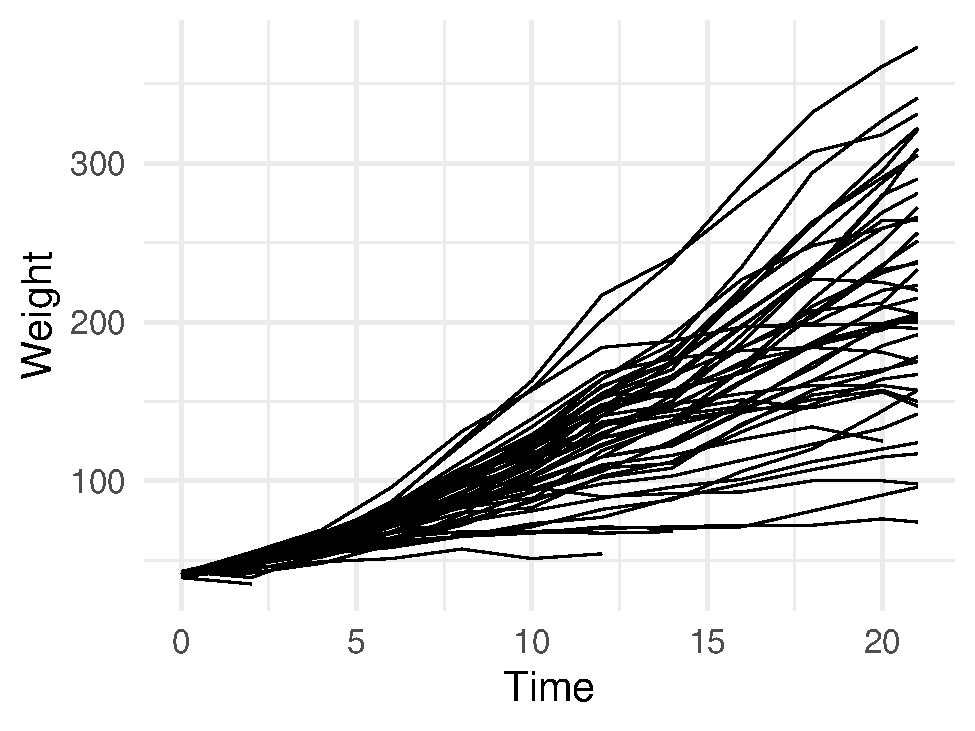
\includegraphics[width=0.8\linewidth]{plotting_r_files/figure-latex/unnamed-chunk-7-1} 

}

\caption{Better looking line plot with colors}\label{fig:unnamed-chunk-7}
\end{figure}

\hypertarget{plotting-using-one-variable-at-a-time}{%
\chapter{Plotting using one variable at a time}\label{plotting-using-one-variable-at-a-time}}

\hypertarget{histograms--plots-the-distribution-of-a-numerical-variable}{%
\section{Histograms- plots the distribution of a numerical variable}\label{histograms--plots-the-distribution-of-a-numerical-variable}}

Note the customizations of the histogram:
1. we colored the bars pretty
2. `alpha' adds transparency to the object, useful when you have overlapping objects, goes from 0 (transparent) to 1 (opaque)

\begin{Shaded}
\begin{Highlighting}[]
\KeywordTok{library}\NormalTok{(ggplot2)}

\KeywordTok{ggplot}\NormalTok{(ChickWeight, }\KeywordTok{aes}\NormalTok{(weight))}\OperatorTok{+}
\StringTok{  }\KeywordTok{geom_histogram}\NormalTok{(}\DataTypeTok{fill=}\StringTok{'cyan4'}\NormalTok{,}\DataTypeTok{color=}\StringTok{'black'}\NormalTok{,}\DataTypeTok{alpha=}\FloatTok{0.5}\NormalTok{)}\OperatorTok{+}
\StringTok{  }\KeywordTok{theme_minimal}\NormalTok{(}\DataTypeTok{base_size =} \DecValTok{20}\NormalTok{)}\OperatorTok{+}
\StringTok{  }\KeywordTok{ylab}\NormalTok{(}\StringTok{"Frequency"}\NormalTok{)}\OperatorTok{+}\StringTok{ }\KeywordTok{xlab}\NormalTok{(}\StringTok{"Weight (g)"}\NormalTok{)}
\end{Highlighting}
\end{Shaded}

\begin{verbatim}
## `stat_bin()` using `bins = 30`. Pick better value with `binwidth`.
\end{verbatim}

\begin{figure}

{\centering 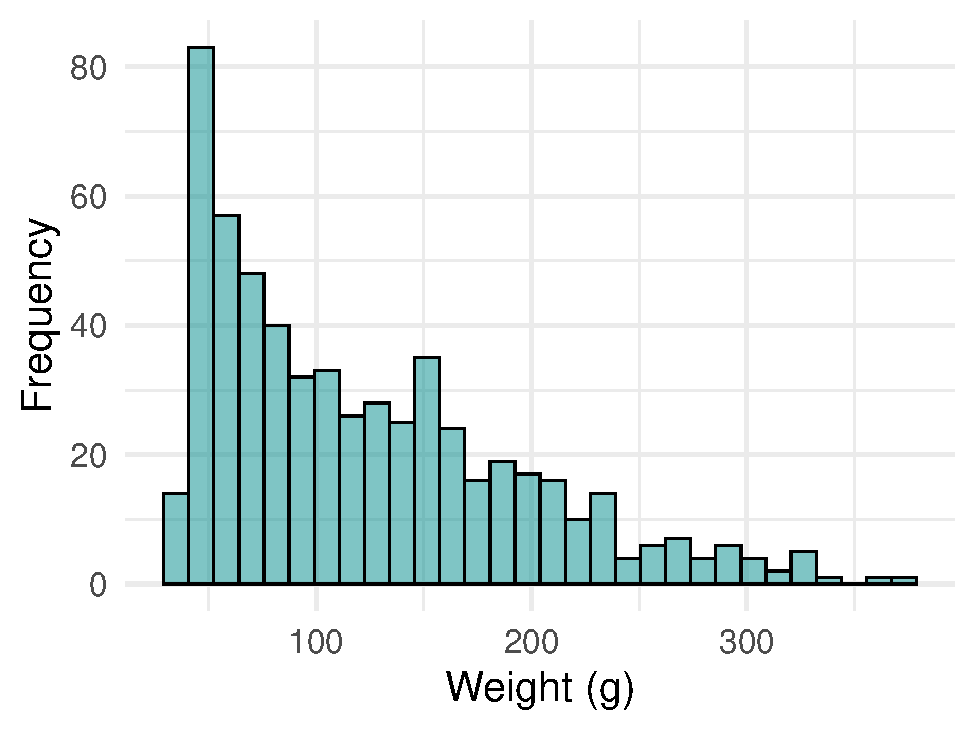
\includegraphics[width=0.8\linewidth]{plotting_r_files/figure-latex/unnamed-chunk-9-1} 

}

\caption{Histogram}\label{fig:unnamed-chunk-9}
\end{figure}

Improving `binwidth' value, it is the number of categories data is divided into and usually defaults to 30, but we can go up and down, let's go to 50 here

\begin{Shaded}
\begin{Highlighting}[]
\KeywordTok{library}\NormalTok{(ggplot2)}

\KeywordTok{ggplot}\NormalTok{(ChickWeight, }\KeywordTok{aes}\NormalTok{(weight))}\OperatorTok{+}
\StringTok{  }\KeywordTok{geom_histogram}\NormalTok{(}\DataTypeTok{fill=}\StringTok{'cyan4'}\NormalTok{,}\DataTypeTok{color=}\StringTok{'black'}\NormalTok{,}\DataTypeTok{alpha=}\FloatTok{0.5}\NormalTok{, }\DataTypeTok{binwidth =} \DecValTok{50}\NormalTok{)}\OperatorTok{+}
\StringTok{  }\KeywordTok{theme_minimal}\NormalTok{(}\DataTypeTok{base_size =} \DecValTok{20}\NormalTok{)}\OperatorTok{+}
\StringTok{  }\KeywordTok{ylab}\NormalTok{(}\StringTok{"Frequency"}\NormalTok{)}\OperatorTok{+}\StringTok{ }\KeywordTok{xlab}\NormalTok{(}\StringTok{"Weight (g)"}\NormalTok{)}
\end{Highlighting}
\end{Shaded}

\begin{figure}

{\centering 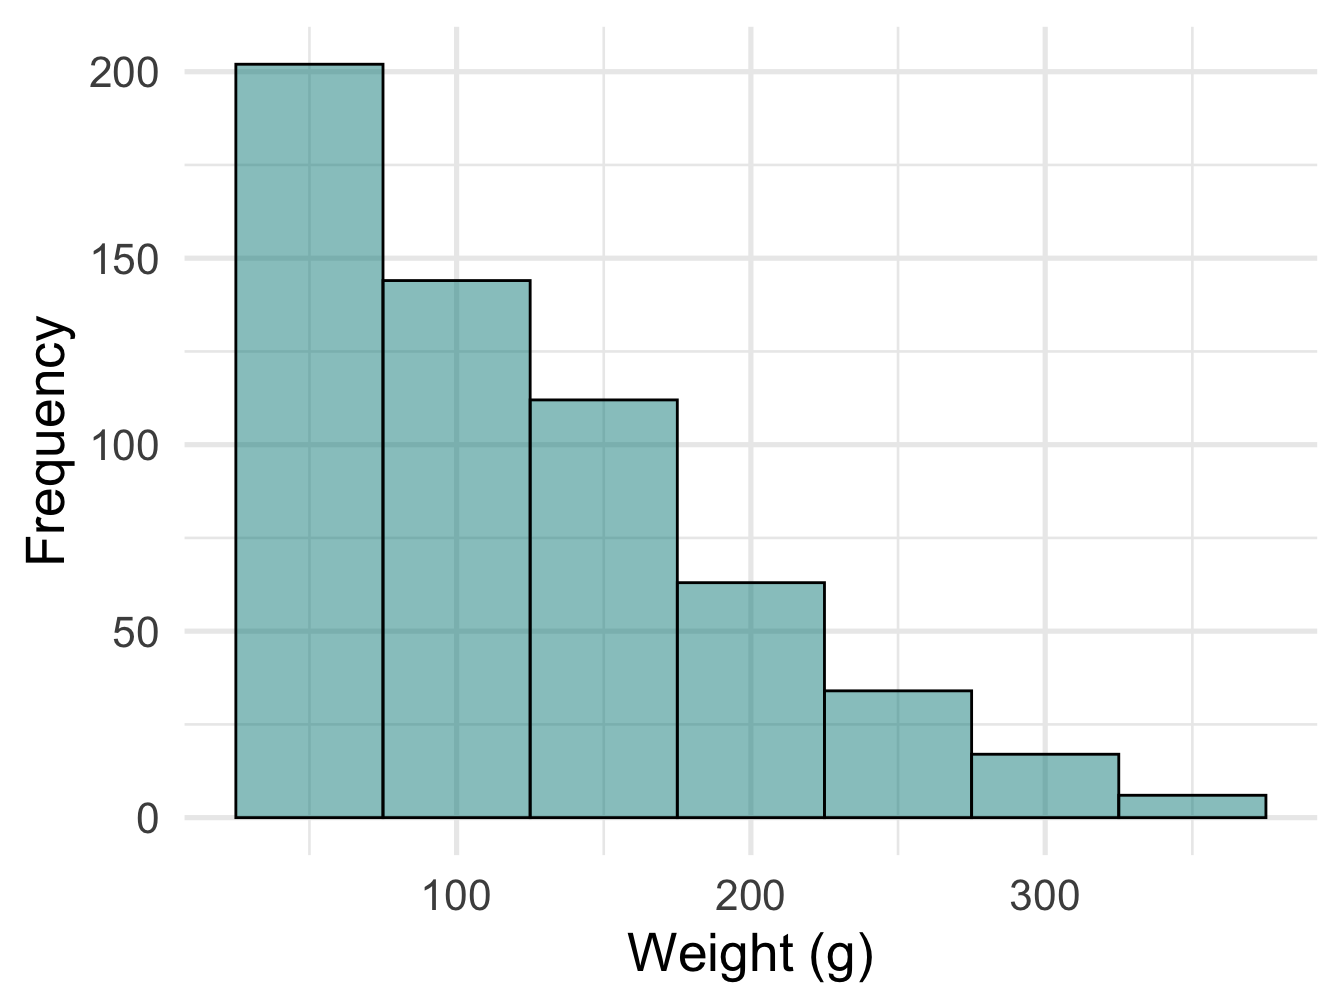
\includegraphics[width=0.8\linewidth]{plotting_r_files/figure-latex/unnamed-chunk-10-1} 

}

\caption{Histogram}\label{fig:unnamed-chunk-10}
\end{figure}

\hypertarget{bar-plots}{%
\section{Bar plots}\label{bar-plots}}

Plot the distribution of a categorical variable

Here we will plot number of chicks following a particular diet.

\begin{Shaded}
\begin{Highlighting}[]
\KeywordTok{library}\NormalTok{(ggplot2)}

\KeywordTok{ggplot}\NormalTok{(ChickWeight, }\KeywordTok{aes}\NormalTok{(}\DataTypeTok{x=}\NormalTok{ Diet))}\OperatorTok{+}
\StringTok{  }\KeywordTok{geom_bar}\NormalTok{(}\DataTypeTok{color=}\StringTok{'orange'}\NormalTok{, }\DataTypeTok{fill=}\StringTok{'lavender'}\NormalTok{)}\OperatorTok{+}
\StringTok{  }\KeywordTok{theme_minimal}\NormalTok{(}\DataTypeTok{base_size =} \DecValTok{20}\NormalTok{)}\OperatorTok{+}
\StringTok{  }\KeywordTok{ylab}\NormalTok{(}\StringTok{"Count"}\NormalTok{)}\OperatorTok{+}\StringTok{ }\KeywordTok{xlab}\NormalTok{(}\StringTok{"Diet"}\NormalTok{)}
\end{Highlighting}
\end{Shaded}

\begin{figure}

{\centering 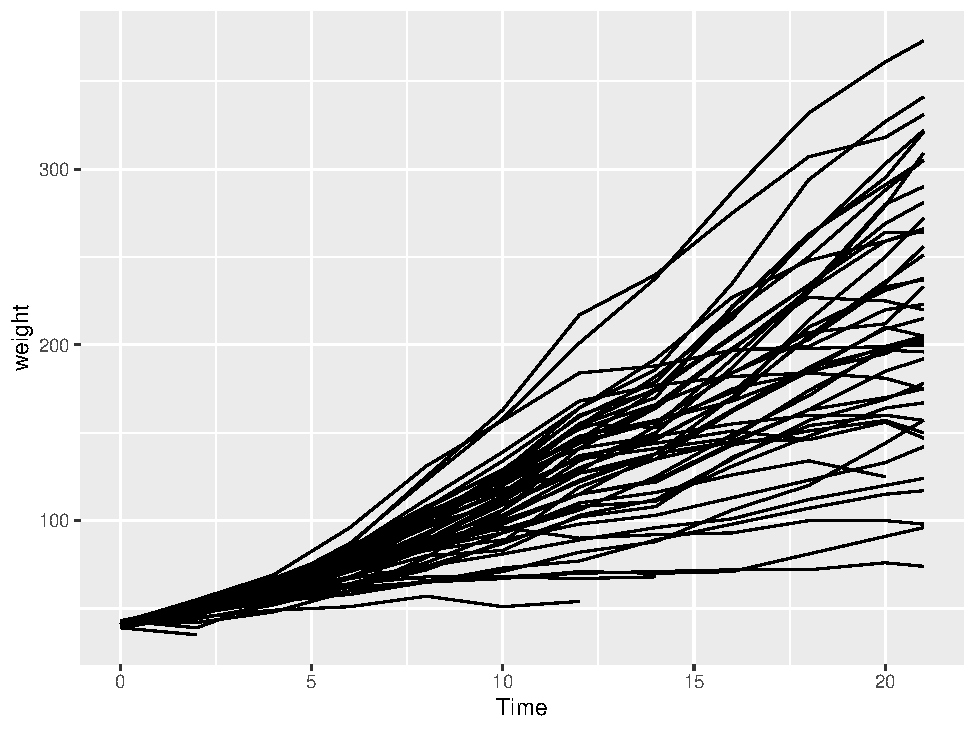
\includegraphics[width=0.8\linewidth]{plotting_r_files/figure-latex/unnamed-chunk-11-1} 

}

\caption{Bar plot}\label{fig:unnamed-chunk-11}
\end{figure}

\hypertarget{ordering-based-on-number-of-counts-from-lowest-to-highest}{%
\section{Ordering based on number of counts from lowest to highest}\label{ordering-based-on-number-of-counts-from-lowest-to-highest}}

Let's bring the magic of dplyer to do so

So we reorganize the data to calcualte number of chicks on each diet type

\begin{Shaded}
\begin{Highlighting}[]
\KeywordTok{library}\NormalTok{(tidyverse)}
\end{Highlighting}
\end{Shaded}

\begin{verbatim}
## -- Attaching packages --------------------------------------- tidyverse 1.3.0 --
\end{verbatim}

\begin{verbatim}
## v tibble  3.0.4     v dplyr   1.0.2
## v tidyr   1.1.2     v stringr 1.4.0
## v readr   1.4.0     v forcats 0.5.0
## v purrr   0.3.4
\end{verbatim}

\begin{verbatim}
## -- Conflicts ------------------------------------------ tidyverse_conflicts() --
## x dplyr::filter() masks stats::filter()
## x dplyr::lag()    masks stats::lag()
\end{verbatim}

\begin{Shaded}
\begin{Highlighting}[]
\NormalTok{reord.chick<-ChickWeight }\OperatorTok\StringTok{ }
\StringTok{ }\KeywordTok{count}\NormalTok{(Diet) }\OperatorTok\StringTok{ }\KeywordTok{arrange}\NormalTok{(n)}
\NormalTok{reord.chick}
\end{Highlighting}
\end{Shaded}

\begin{verbatim}
##   Diet   n
## 1    4 118
## 2    2 120
## 3    3 120
## 4    1 220
\end{verbatim}

Here we plot using geom\_col function where heights represents the value of the data and requires y aesthetics. We can use geom\_text function to add the label to each column and use vjust to move the labels up and down

\begin{Shaded}
\begin{Highlighting}[]
\KeywordTok{library}\NormalTok{(ggplot2)}

\KeywordTok{ggplot}\NormalTok{(reord.chick, }\KeywordTok{aes}\NormalTok{(}\DataTypeTok{x=} \KeywordTok{reorder}\NormalTok{(Diet,n), }\DataTypeTok{y=}\NormalTok{n))}\OperatorTok{+}
\StringTok{  }\KeywordTok{geom_col}\NormalTok{(}\DataTypeTok{color=}\StringTok{'orange'}\NormalTok{, }\DataTypeTok{fill=}\StringTok{'lavender'}\NormalTok{)}\OperatorTok{+}
\StringTok{  }\KeywordTok{geom_text}\NormalTok{(}\KeywordTok{aes}\NormalTok{(}\DataTypeTok{label=}\NormalTok{n), }\DataTypeTok{vjust=}\OperatorTok{-}\FloatTok{0.7}\NormalTok{)}\OperatorTok{+}
\StringTok{  }\KeywordTok{theme_minimal}\NormalTok{(}\DataTypeTok{base_size =} \DecValTok{20}\NormalTok{)}\OperatorTok{+}
\StringTok{  }\KeywordTok{ylab}\NormalTok{(}\StringTok{"Count"}\NormalTok{)}\OperatorTok{+}\StringTok{ }\KeywordTok{xlab}\NormalTok{(}\StringTok{"Diet"}\NormalTok{)}
\end{Highlighting}
\end{Shaded}

\begin{figure}

{\centering 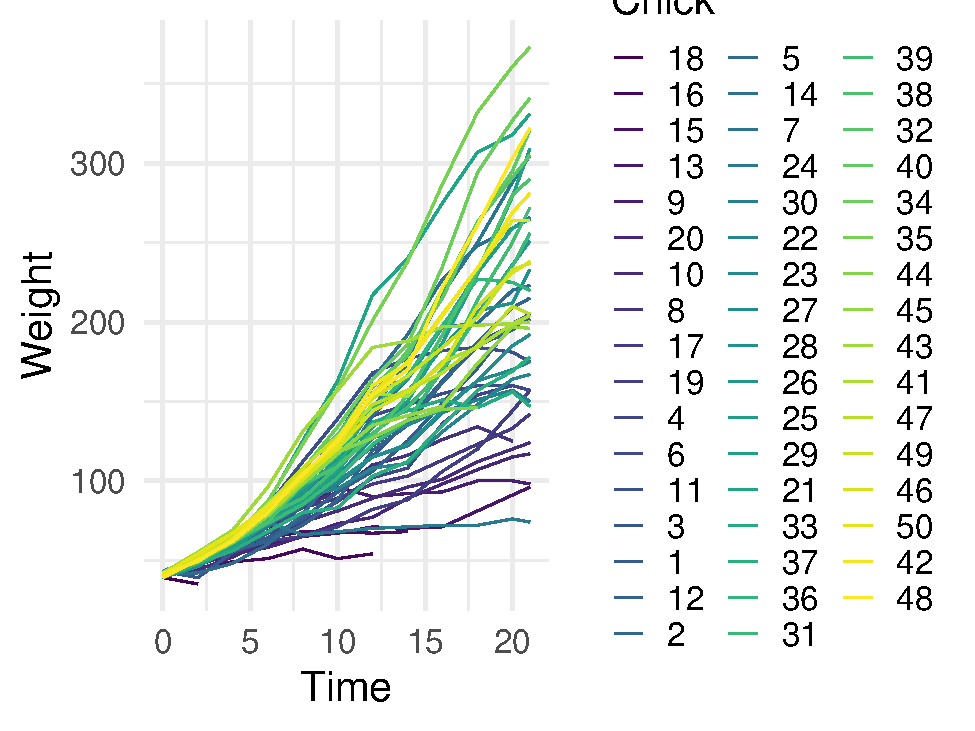
\includegraphics[width=0.8\linewidth]{plotting_r_files/figure-latex/unnamed-chunk-13-1} 

}

\caption{Bar plot with labels}\label{fig:unnamed-chunk-13}
\end{figure}

\hypertarget{adding-percentages}{%
\section{Adding percentages}\label{adding-percentages}}

Here we also get more adventerous with data wrangling and create new columns and plot them within the same pipe

\begin{Shaded}
\begin{Highlighting}[]
\NormalTok{ChickWeight }\OperatorTok\StringTok{ }
\StringTok{  }\KeywordTok{count}\NormalTok{(Diet) }\OperatorTok\StringTok{ }\KeywordTok{arrange}\NormalTok{(n) }\OperatorTok\StringTok{ }
\KeywordTok{mutate}\NormalTok{(}\DataTypeTok{percent =}\NormalTok{ n }\OperatorTok{/}\StringTok{ }\KeywordTok{sum}\NormalTok{(n),}
         \DataTypeTok{percentlabel =} \KeywordTok{paste0}\NormalTok{(}\KeywordTok{round}\NormalTok{(percent}\OperatorTok{*}\DecValTok{100}\NormalTok{), }\StringTok{"%"}\NormalTok{)) }\OperatorTok\StringTok{ }

\KeywordTok{ggplot}\NormalTok{( }\KeywordTok{aes}\NormalTok{(}\DataTypeTok{x=} \KeywordTok{reorder}\NormalTok{(Diet,percent), }\DataTypeTok{y=}\NormalTok{percent))}\OperatorTok{+}
\StringTok{  }\KeywordTok{geom_col}\NormalTok{(}\DataTypeTok{color=}\StringTok{'orange'}\NormalTok{, }\DataTypeTok{fill=}\StringTok{'lavender'}\NormalTok{)}\OperatorTok{+}
\StringTok{  }\KeywordTok{geom_text}\NormalTok{(}\KeywordTok{aes}\NormalTok{(}\DataTypeTok{label=}\NormalTok{percentlabel), }\DataTypeTok{vjust=}\OperatorTok{-}\FloatTok{0.7}\NormalTok{)}\OperatorTok{+}
\StringTok{  }\KeywordTok{theme_minimal}\NormalTok{(}\DataTypeTok{base_size =} \DecValTok{20}\NormalTok{)}\OperatorTok{+}
\StringTok{  }\KeywordTok{ylab}\NormalTok{(}\StringTok{"Count"}\NormalTok{)}\OperatorTok{+}\StringTok{ }\KeywordTok{xlab}\NormalTok{(}\StringTok{"Diet"}\NormalTok{)}
\end{Highlighting}
\end{Shaded}

\begin{figure}

{\centering 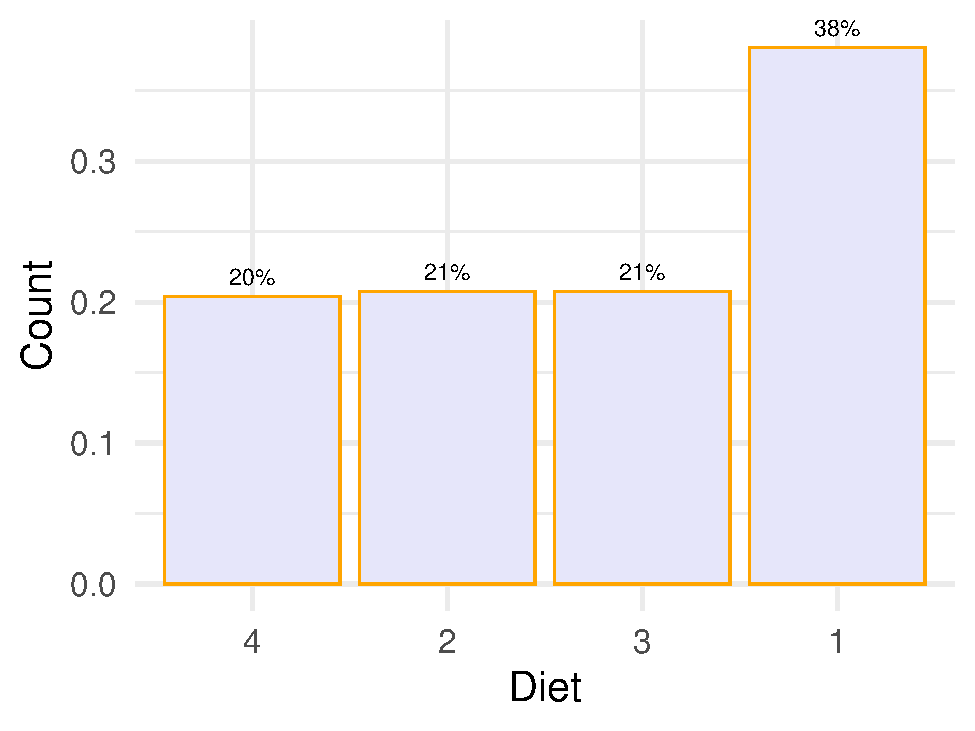
\includegraphics[width=0.8\linewidth]{plotting_r_files/figure-latex/unnamed-chunk-14-1} 

}

\caption{Bar plot with percent labels}\label{fig:unnamed-chunk-14}
\end{figure}

\hypertarget{pie-chart}{%
\section{pie chart}\label{pie-chart}}

\begin{Shaded}
\begin{Highlighting}[]
\KeywordTok{library}\NormalTok{(ggplot2)}

\KeywordTok{ggplot}\NormalTok{(reord.chick, }\KeywordTok{aes}\NormalTok{(}\DataTypeTok{x=} \KeywordTok{reorder}\NormalTok{(Diet,n), }\DataTypeTok{y=}\NormalTok{n,}\DataTypeTok{fill=}\NormalTok{Diet))}\OperatorTok{+}
\StringTok{  }\KeywordTok{geom_col}\NormalTok{(}\DataTypeTok{width =} \DecValTok{1}\NormalTok{, }
           \DataTypeTok{stat =} \StringTok{"identity"}\NormalTok{, }
           \DataTypeTok{color =} \StringTok{"black"}\NormalTok{) }\OperatorTok{+}
\StringTok{  }\KeywordTok{geom_text}\NormalTok{(}\KeywordTok{aes}\NormalTok{(}\DataTypeTok{label=}\NormalTok{n), }\DataTypeTok{vjust=}\OperatorTok{-}\FloatTok{0.7}\NormalTok{)}\OperatorTok{+}
\StringTok{  }\KeywordTok{theme_minimal}\NormalTok{(}\DataTypeTok{base_size =} \DecValTok{20}\NormalTok{)}\OperatorTok{+}
\StringTok{  }\KeywordTok{coord_polar}\NormalTok{(}\StringTok{"y"}\NormalTok{, }
              \DataTypeTok{start =} \DecValTok{0}\NormalTok{, }
              \DataTypeTok{direction =} \DecValTok{-1}\NormalTok{) }\OperatorTok{+}
\StringTok{  }\KeywordTok{theme_void}\NormalTok{() }\OperatorTok{+}
\StringTok{  }\KeywordTok{ylab}\NormalTok{(}\StringTok{"Count"}\NormalTok{)}\OperatorTok{+}\StringTok{ }\KeywordTok{xlab}\NormalTok{(}\StringTok{"Diet"}\NormalTok{)}
\end{Highlighting}
\end{Shaded}

\begin{verbatim}
## Warning: Ignoring unknown parameters: stat
\end{verbatim}

\begin{figure}

{\centering 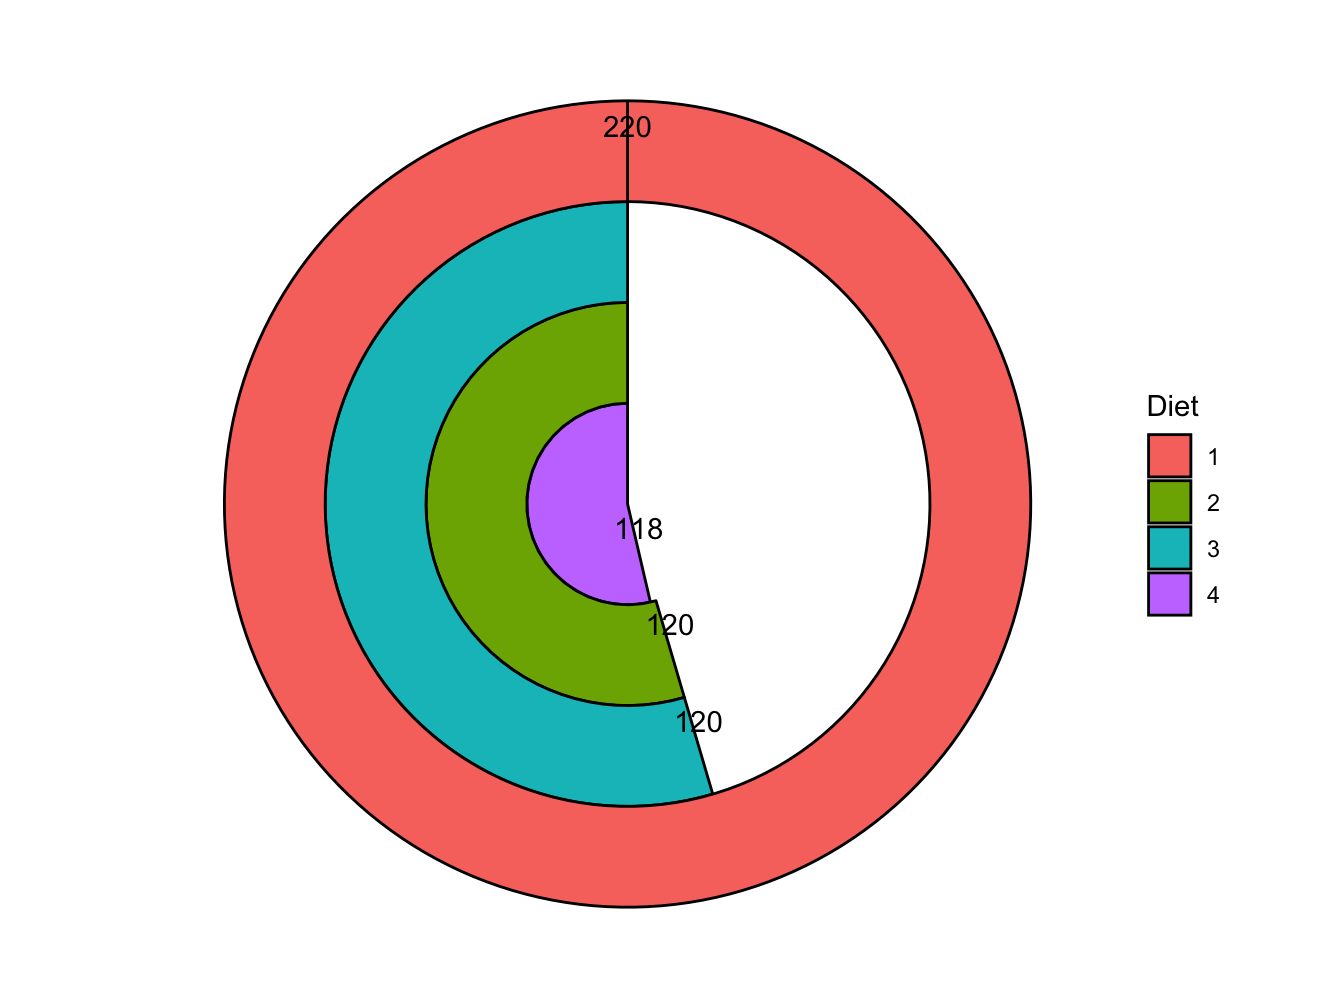
\includegraphics[width=0.8\linewidth]{plotting_r_files/figure-latex/unnamed-chunk-15-1} 

}

\caption{Pie chart with labels }\label{fig:unnamed-chunk-15}
\end{figure}

\hypertarget{multivariate-data}{%
\chapter{Multivariate data}\label{multivariate-data}}

Now we will plot using multiple variables

Let's use diamond dataset from tidyr

\begin{Shaded}
\begin{Highlighting}[]
\KeywordTok{data}\NormalTok{(}\StringTok{"diamonds"}\NormalTok{)}
\KeywordTok{head}\NormalTok{(diamonds)}
\end{Highlighting}
\end{Shaded}

\begin{verbatim}
## # A tibble: 6 x 10
##   carat cut       color clarity depth table price     x     y     z
##   <dbl> <ord>     <ord> <ord>   <dbl> <dbl> <int> <dbl> <dbl> <dbl>
## 1 0.23  Ideal     E     SI2      61.5    55   326  3.95  3.98  2.43
## 2 0.21  Premium   E     SI1      59.8    61   326  3.89  3.84  2.31
## 3 0.23  Good      E     VS1      56.9    65   327  4.05  4.07  2.31
## 4 0.290 Premium   I     VS2      62.4    58   334  4.2   4.23  2.63
## 5 0.31  Good      J     SI2      63.3    58   335  4.34  4.35  2.75
## 6 0.24  Very Good J     VVS2     62.8    57   336  3.94  3.96  2.48
\end{verbatim}

\hypertarget{bar-plot-with-categories-plot-depth-by-cut}{%
\section{Bar plot with categories, plot depth by cut}\label{bar-plot-with-categories-plot-depth-by-cut}}

\begin{Shaded}
\begin{Highlighting}[]
\KeywordTok{ggplot}\NormalTok{(diamonds)}\OperatorTok{+}
\StringTok{ }\KeywordTok{geom_bar}\NormalTok{(}\KeywordTok{aes}\NormalTok{(}\DataTypeTok{x=}\NormalTok{ cut, }\DataTypeTok{fill=}\NormalTok{color))}\OperatorTok{+}
\StringTok{  }\KeywordTok{theme_minimal}\NormalTok{(}\DataTypeTok{base_size =} \DecValTok{20}\NormalTok{)}\OperatorTok{+}
\StringTok{  }\KeywordTok{ylab}\NormalTok{(}\StringTok{"Count"}\NormalTok{)}\OperatorTok{+}\StringTok{ }\KeywordTok{xlab}\NormalTok{(}\StringTok{"Cut"}\NormalTok{)}
\end{Highlighting}
\end{Shaded}

\begin{figure}

{\centering 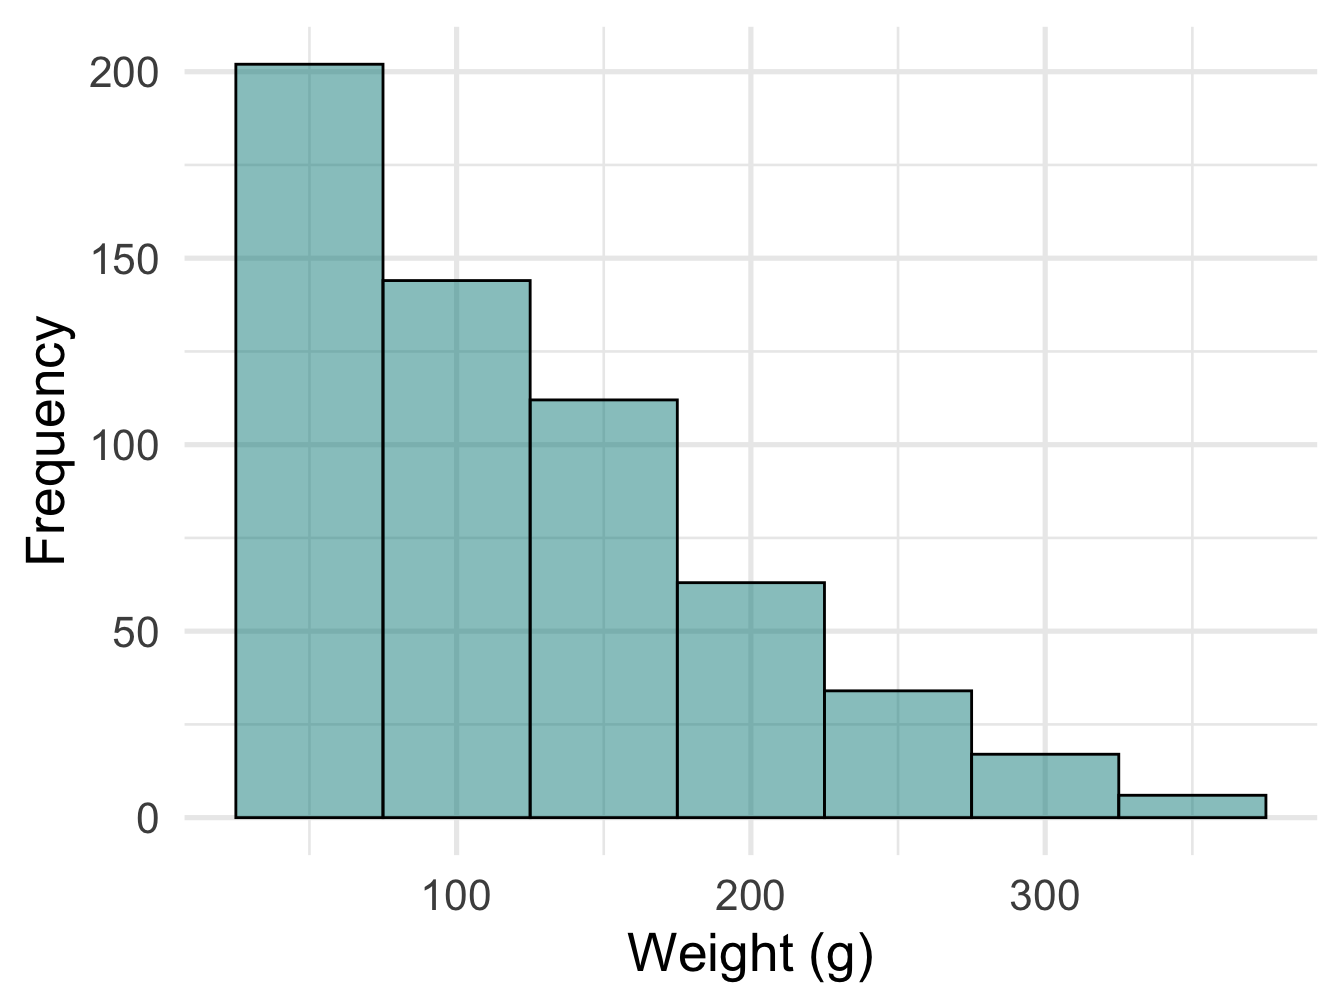
\includegraphics[width=0.8\linewidth]{plotting_r_files/figure-latex/unnamed-chunk-17-1} 

}

\caption{Bar plot with grouping}\label{fig:unnamed-chunk-17}
\end{figure}

\hypertarget{bar-plot-with-categories-side-by-side}{%
\section{Bar plot with categories, side by side}\label{bar-plot-with-categories-side-by-side}}

\begin{Shaded}
\begin{Highlighting}[]
\KeywordTok{ggplot}\NormalTok{(diamonds)}\OperatorTok{+}
\StringTok{ }\KeywordTok{geom_bar}\NormalTok{(}\KeywordTok{aes}\NormalTok{(}\DataTypeTok{x=}\NormalTok{ cut, }\DataTypeTok{fill=}\NormalTok{color),}\DataTypeTok{position =} \KeywordTok{position_dodge}\NormalTok{())}\OperatorTok{+}
\StringTok{  }\KeywordTok{theme_minimal}\NormalTok{(}\DataTypeTok{base_size =} \DecValTok{20}\NormalTok{)}\OperatorTok{+}
\StringTok{  }\KeywordTok{ylab}\NormalTok{(}\StringTok{"Count"}\NormalTok{)}\OperatorTok{+}\StringTok{ }\KeywordTok{xlab}\NormalTok{(}\StringTok{"Cut"}\NormalTok{)}
\end{Highlighting}
\end{Shaded}

\begin{figure}

{\centering 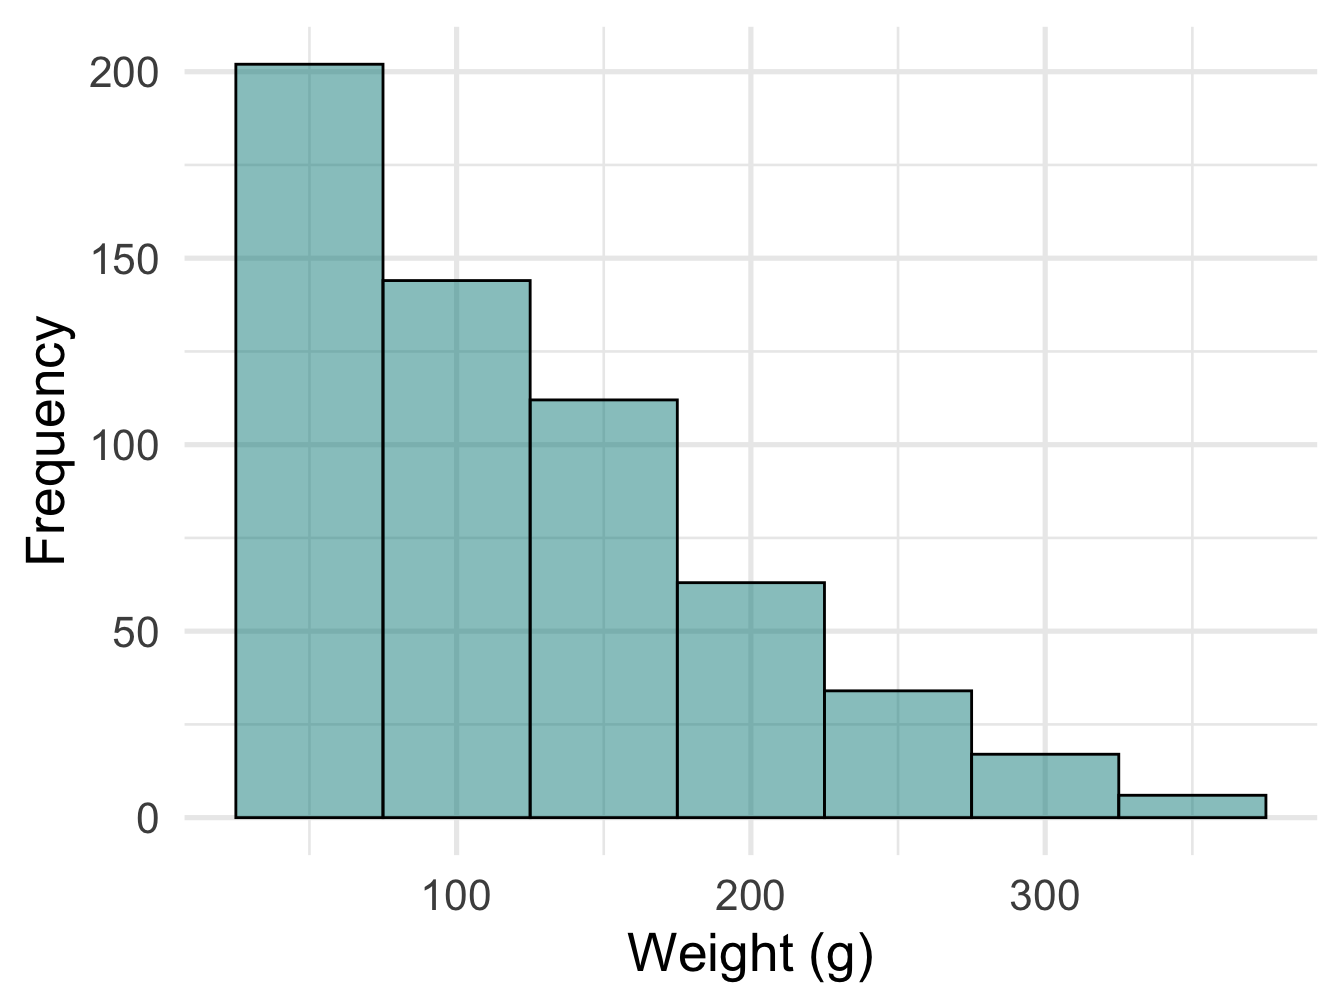
\includegraphics[width=0.8\linewidth]{plotting_r_files/figure-latex/unnamed-chunk-18-1} 

}

\caption{Bar plot with grouping}\label{fig:unnamed-chunk-18}
\end{figure}

\hypertarget{segemented-bar-plot-appealing-viz}{%
\section{Segemented bar plot, appealing viz}\label{segemented-bar-plot-appealing-viz}}

\begin{Shaded}
\begin{Highlighting}[]
\NormalTok{diamonds }\OperatorTok
\StringTok{  }\KeywordTok{group_by}\NormalTok{(cut, color) }\OperatorTok
\StringTok{  }\KeywordTok{summarize}\NormalTok{(}\DataTypeTok{n =} \KeywordTok{n}\NormalTok{()) }\OperatorTok\StringTok{ }
\StringTok{  }\KeywordTok{mutate}\NormalTok{(}\DataTypeTok{prct =}\NormalTok{ n}\OperatorTok{/}\KeywordTok{sum}\NormalTok{(n),}
         \DataTypeTok{label =}\NormalTok{ scales}\OperatorTok{::}\KeywordTok{percent}\NormalTok{(prct)) }\OperatorTok\StringTok{ }
\StringTok{         }\KeywordTok{ggplot}\NormalTok{()}\OperatorTok{+}
\StringTok{          }\KeywordTok{geom_col}\NormalTok{(}\KeywordTok{aes}\NormalTok{(}\DataTypeTok{x=}\NormalTok{cut,}\DataTypeTok{y=}\NormalTok{prct,}\DataTypeTok{fill=}\NormalTok{color),}\DataTypeTok{position=}\StringTok{'fill'}\NormalTok{)}\OperatorTok{+}
\StringTok{          }\KeywordTok{geom_text}\NormalTok{(}\KeywordTok{aes}\NormalTok{(}\DataTypeTok{x=}\NormalTok{cut,}\DataTypeTok{y=}\NormalTok{prct,}\DataTypeTok{label =}\NormalTok{ label), }
            \DataTypeTok{size =} \DecValTok{3}\NormalTok{, }
            \DataTypeTok{position =} \KeywordTok{position_stack}\NormalTok{(}\DataTypeTok{vjust =} \FloatTok{0.5}\NormalTok{)) }\OperatorTok{+}
\StringTok{             }\KeywordTok{theme_minimal}\NormalTok{(}\DataTypeTok{base_size =} \DecValTok{20}\NormalTok{)}\OperatorTok{+}
\StringTok{  }\KeywordTok{ylab}\NormalTok{(}\StringTok{"Percentage"}\NormalTok{)}\OperatorTok{+}\StringTok{ }\KeywordTok{xlab}\NormalTok{(}\StringTok{"Cut"}\NormalTok{)}
\end{Highlighting}
\end{Shaded}

\begin{verbatim}
## `summarise()` regrouping output by 'cut' (override with `.groups` argument)
\end{verbatim}

\begin{figure}

{\centering 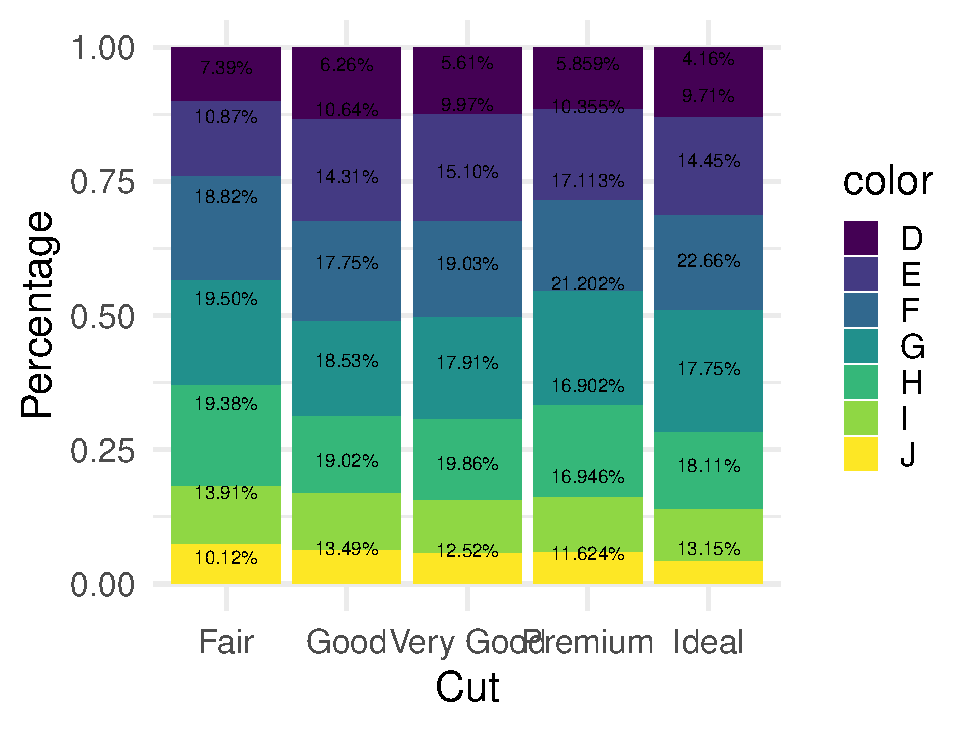
\includegraphics[width=0.8\linewidth]{plotting_r_files/figure-latex/unnamed-chunk-19-1} 

}

\caption{Bar plot with grouping}\label{fig:unnamed-chunk-19}
\end{figure}

\hypertarget{scatter-plot}{%
\section{Scatter plot}\label{scatter-plot}}

\begin{Shaded}
\begin{Highlighting}[]
         \KeywordTok{ggplot}\NormalTok{(diamonds)}\OperatorTok{+}
\StringTok{          }\KeywordTok{geom_point}\NormalTok{(}\KeywordTok{aes}\NormalTok{(}\DataTypeTok{x=}\NormalTok{carat,}\DataTypeTok{y=}\NormalTok{price,}\DataTypeTok{color=}\NormalTok{color))}\OperatorTok{+}
\StringTok{  }\KeywordTok{theme_bw}\NormalTok{()}\OperatorTok{+}
\StringTok{  }\KeywordTok{xlab}\NormalTok{(}\StringTok{"Carat"}\NormalTok{)}\OperatorTok{+}\StringTok{ }\KeywordTok{ylab}\NormalTok{(}\StringTok{"Price"}\NormalTok{)}
\end{Highlighting}
\end{Shaded}

\begin{figure}

{\centering 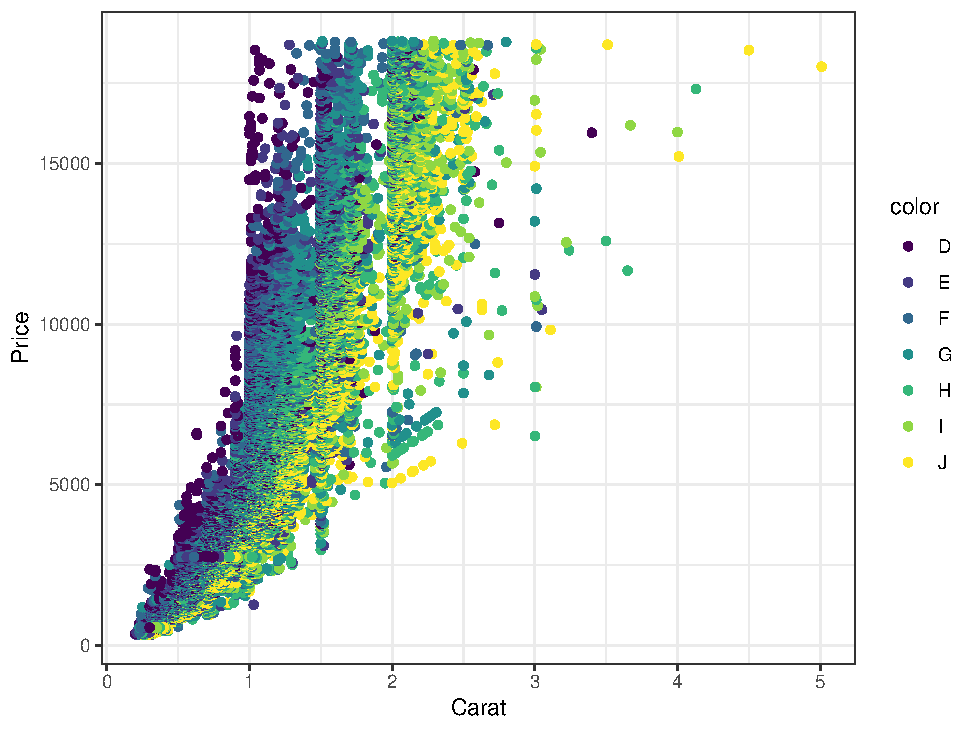
\includegraphics[width=0.8\linewidth]{plotting_r_files/figure-latex/unnamed-chunk-20-1} 

}

\caption{Scatter plot with grouping}\label{fig:unnamed-chunk-20}
\end{figure}

Let's see if the depth is related to price

\begin{Shaded}
\begin{Highlighting}[]
         \KeywordTok{ggplot}\NormalTok{(diamonds)}\OperatorTok{+}
\StringTok{          }\KeywordTok{geom_point}\NormalTok{(}\KeywordTok{aes}\NormalTok{(}\DataTypeTok{x=}\NormalTok{carat,}\DataTypeTok{y=}\NormalTok{price,}\DataTypeTok{color=}\NormalTok{color))}\OperatorTok{+}
\StringTok{  }\KeywordTok{geom_smooth}\NormalTok{(}\KeywordTok{aes}\NormalTok{(}\DataTypeTok{x=}\NormalTok{carat,}\DataTypeTok{y=}\NormalTok{price,}\DataTypeTok{color=}\NormalTok{color),}\DataTypeTok{method=}\StringTok{'lm'}\NormalTok{)}\OperatorTok{+}
\StringTok{  }\KeywordTok{theme_bw}\NormalTok{()}\OperatorTok{+}
\StringTok{  }\KeywordTok{ylab}\NormalTok{(}\StringTok{"Price"}\NormalTok{)}\OperatorTok{+}\StringTok{ }\KeywordTok{xlab}\NormalTok{(}\StringTok{"Price"}\NormalTok{)}
\end{Highlighting}
\end{Shaded}

\begin{verbatim}
## `geom_smooth()` using formula 'y ~ x'
\end{verbatim}

\begin{figure}

{\centering 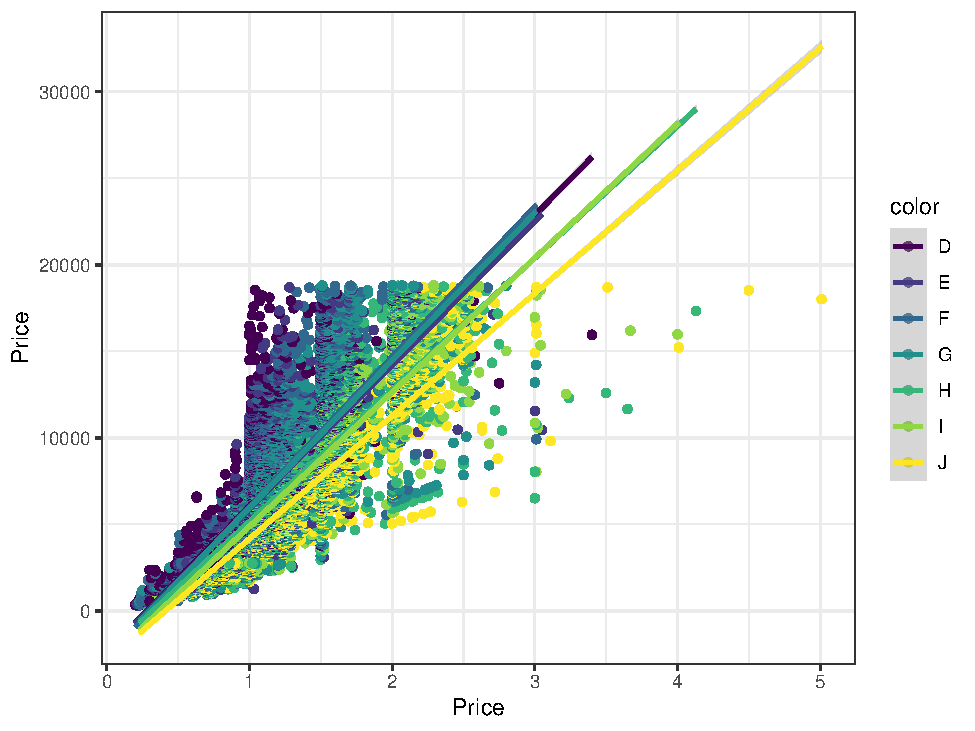
\includegraphics[width=0.8\linewidth]{plotting_r_files/figure-latex/unnamed-chunk-21-1} 

}

\caption{Scatter plot with grouping and smooth line}\label{fig:unnamed-chunk-21}
\end{figure}

\hypertarget{grouping-using-facets}{%
\section{Grouping using facets}\label{grouping-using-facets}}

\begin{Shaded}
\begin{Highlighting}[]
         \KeywordTok{ggplot}\NormalTok{(diamonds)}\OperatorTok{+}
\StringTok{          }\KeywordTok{geom_point}\NormalTok{(}\KeywordTok{aes}\NormalTok{(}\DataTypeTok{x=}\NormalTok{carat,}\DataTypeTok{y=}\NormalTok{price))}\OperatorTok{+}
\StringTok{  }\KeywordTok{geom_smooth}\NormalTok{(}\KeywordTok{aes}\NormalTok{(}\DataTypeTok{x=}\NormalTok{carat,}\DataTypeTok{y=}\NormalTok{price),}\DataTypeTok{method=}\StringTok{'lm'}\NormalTok{)}\OperatorTok{+}
\StringTok{  }\KeywordTok{facet_wrap}\NormalTok{(}\OperatorTok{~}\NormalTok{color)}\OperatorTok{+}
\StringTok{  }\KeywordTok{theme_bw}\NormalTok{()}\OperatorTok{+}
\StringTok{  }\KeywordTok{ylab}\NormalTok{(}\StringTok{"Carat"}\NormalTok{)}\OperatorTok{+}\StringTok{ }\KeywordTok{xlab}\NormalTok{(}\StringTok{"Price"}\NormalTok{)}
\end{Highlighting}
\end{Shaded}

\begin{verbatim}
## `geom_smooth()` using formula 'y ~ x'
\end{verbatim}

\begin{figure}

{\centering 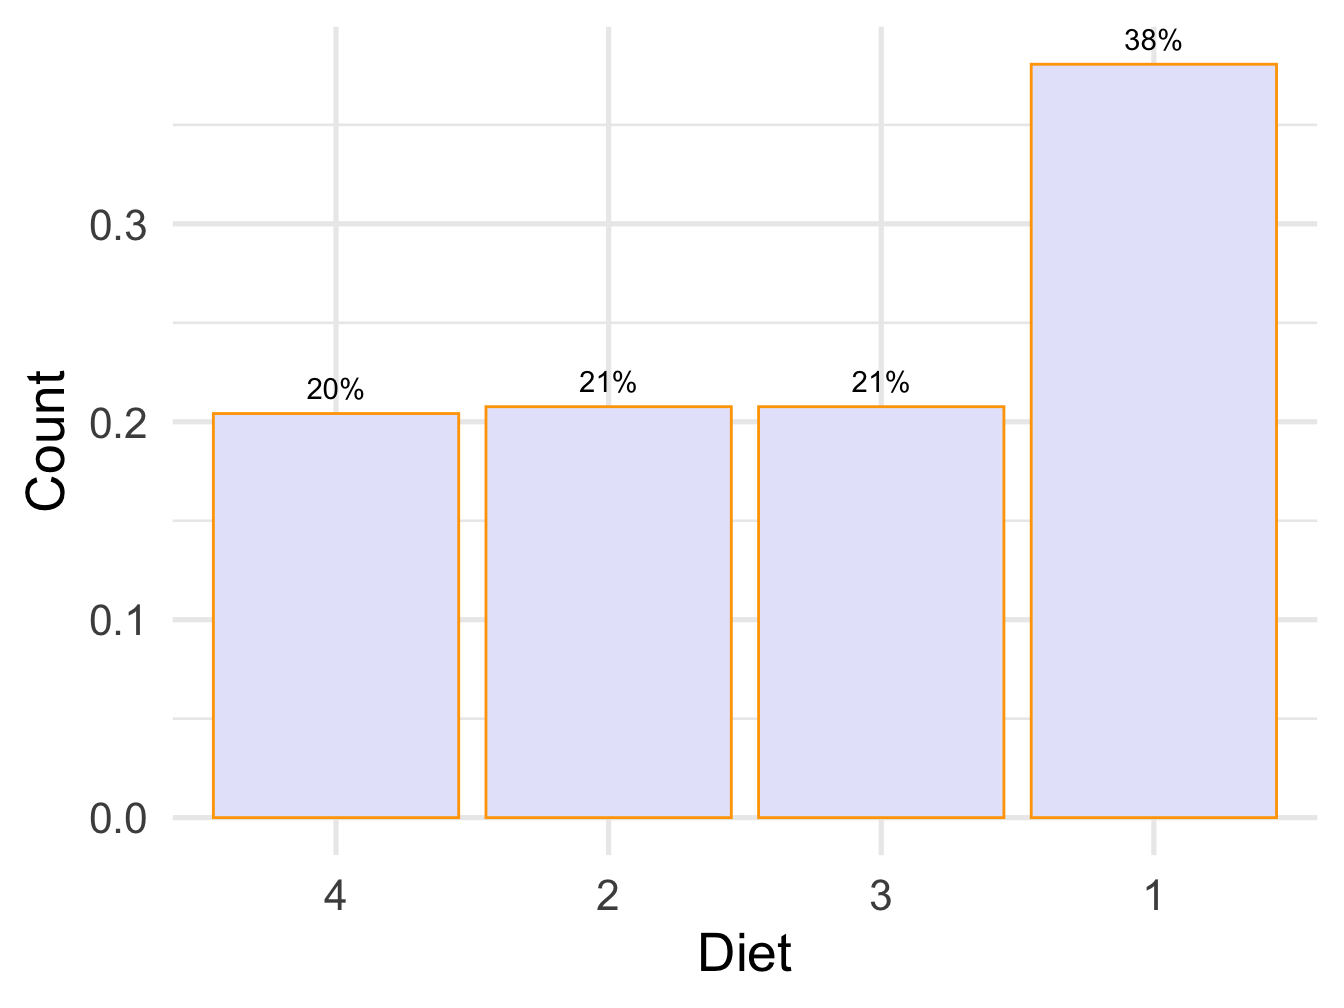
\includegraphics[width=0.8\linewidth]{plotting_r_files/figure-latex/unnamed-chunk-22-1} 

}

\caption{Scatter plot with facets and smooth line}\label{fig:unnamed-chunk-22}
\end{figure}

\hypertarget{grouping-using-facets-1}{%
\section{Grouping using facets}\label{grouping-using-facets-1}}

\begin{Shaded}
\begin{Highlighting}[]
\NormalTok{diamonds2<-diamonds}
\KeywordTok{levels}\NormalTok{(diamonds2}\OperatorTok{$}\NormalTok{color)}
\end{Highlighting}
\end{Shaded}

\begin{verbatim}
## [1] "D" "E" "F" "G" "H" "I" "J"
\end{verbatim}

\begin{Shaded}
\begin{Highlighting}[]
\NormalTok{diamonds2}\OperatorTok{$}\NormalTok{color<-}\StringTok{ }\KeywordTok{factor}\NormalTok{(diamonds2}\OperatorTok{$}\NormalTok{color, }\DataTypeTok{levels =}\KeywordTok{c}\NormalTok{(}\StringTok{"D"}\NormalTok{ ,}\StringTok{"E"}\NormalTok{ ,}\StringTok{"F"}\NormalTok{ ,}\StringTok{"G"}\NormalTok{, }\StringTok{"H"}\NormalTok{, }\StringTok{"I"}\NormalTok{, }\StringTok{"J"}\NormalTok{), }
                         \DataTypeTok{labels=}\KeywordTok{c}\NormalTok{(}\StringTok{"Red"}\NormalTok{,}\StringTok{"Blue"}\NormalTok{,}\StringTok{"Orange"}\NormalTok{,}\StringTok{"Pink"}\NormalTok{,}\StringTok{"Indigo"}\NormalTok{,}\StringTok{"Jade"}\NormalTok{,}\StringTok{"Orange"}\NormalTok{))}
         \KeywordTok{ggplot}\NormalTok{(diamonds2)}\OperatorTok{+}
\StringTok{          }\KeywordTok{geom_point}\NormalTok{(}\KeywordTok{aes}\NormalTok{(}\DataTypeTok{x=}\NormalTok{carat,}\DataTypeTok{y=}\NormalTok{price))}\OperatorTok{+}
\StringTok{  }\KeywordTok{geom_smooth}\NormalTok{(}\KeywordTok{aes}\NormalTok{(}\DataTypeTok{x=}\NormalTok{carat,}\DataTypeTok{y=}\NormalTok{price),}\DataTypeTok{method=}\StringTok{'lm'}\NormalTok{)}\OperatorTok{+}
\StringTok{  }\KeywordTok{facet_wrap}\NormalTok{(}\OperatorTok{~}\NormalTok{color)}\OperatorTok{+}
\StringTok{  }\KeywordTok{theme_bw}\NormalTok{()}\OperatorTok{+}
\StringTok{  }\KeywordTok{ylab}\NormalTok{(}\StringTok{"Carat"}\NormalTok{)}\OperatorTok{+}\StringTok{ }\KeywordTok{xlab}\NormalTok{(}\StringTok{"Price"}\NormalTok{)}
\end{Highlighting}
\end{Shaded}

\begin{verbatim}
## `geom_smooth()` using formula 'y ~ x'
\end{verbatim}

\begin{figure}

{\centering 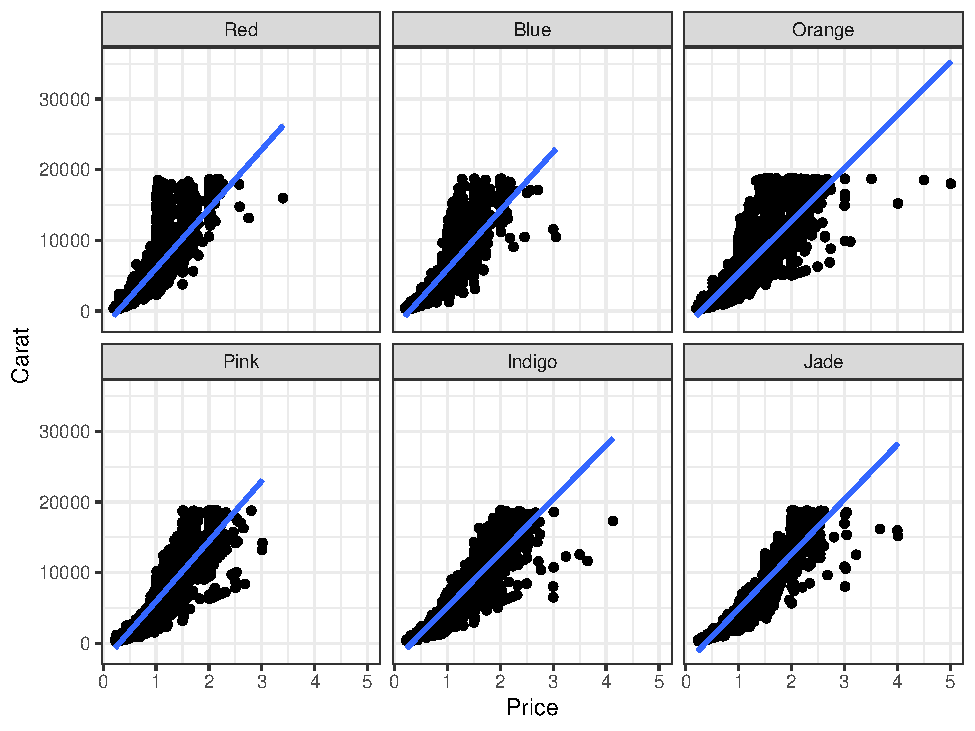
\includegraphics[width=0.8\linewidth]{plotting_r_files/figure-latex/unnamed-chunk-23-1} 

}

\caption{Scatter plot with facets and different labels}\label{fig:unnamed-chunk-23}
\end{figure}

\hypertarget{publication-style-figures-and-saving}{%
\chapter{Publication style figures and saving}\label{publication-style-figures-and-saving}}

`ggpubr' package is wondeful to create publication quality figures

\begin{Shaded}
\begin{Highlighting}[]
\NormalTok{diamonds2<-diamonds}
\KeywordTok{levels}\NormalTok{(diamonds2}\OperatorTok{$}\NormalTok{color)}
\end{Highlighting}
\end{Shaded}

\begin{verbatim}
## [1] "D" "E" "F" "G" "H" "I" "J"
\end{verbatim}

\begin{Shaded}
\begin{Highlighting}[]
\NormalTok{diamonds2}\OperatorTok{$}\NormalTok{color<-}\StringTok{ }\KeywordTok{factor}\NormalTok{(diamonds2}\OperatorTok{$}\NormalTok{color, }\DataTypeTok{levels =}\KeywordTok{c}\NormalTok{(}\StringTok{"D"}\NormalTok{ ,}\StringTok{"E"}\NormalTok{ ,}\StringTok{"F"}\NormalTok{ ,}\StringTok{"G"}\NormalTok{, }\StringTok{"H"}\NormalTok{, }\StringTok{"I"}\NormalTok{, }\StringTok{"J"}\NormalTok{), }
                         \DataTypeTok{labels=}\KeywordTok{c}\NormalTok{(}\StringTok{"Red"}\NormalTok{,}\StringTok{"Blue"}\NormalTok{,}\StringTok{"Orange"}\NormalTok{,}\StringTok{"Pink"}\NormalTok{,}\StringTok{"Indigo"}\NormalTok{,}\StringTok{"Jade"}\NormalTok{,}\StringTok{"Orange"}\NormalTok{))}
         \KeywordTok{ggplot}\NormalTok{(diamonds2)}\OperatorTok{+}
\StringTok{          }\KeywordTok{geom_point}\NormalTok{(}\KeywordTok{aes}\NormalTok{(}\DataTypeTok{x=}\NormalTok{carat,}\DataTypeTok{y=}\NormalTok{price))}\OperatorTok{+}
\StringTok{  }\KeywordTok{geom_smooth}\NormalTok{(}\KeywordTok{aes}\NormalTok{(}\DataTypeTok{x=}\NormalTok{carat,}\DataTypeTok{y=}\NormalTok{price),}\DataTypeTok{method=}\StringTok{'lm'}\NormalTok{)}\OperatorTok{+}
\StringTok{  }\KeywordTok{facet_wrap}\NormalTok{(}\OperatorTok{~}\NormalTok{color)}\OperatorTok{+}
\StringTok{  }\NormalTok{ggpubr}\OperatorTok{::}\KeywordTok{theme_pubr}\NormalTok{(}\DataTypeTok{base_size=}\DecValTok{22}\NormalTok{)}\OperatorTok{+}
\StringTok{           }
\StringTok{  }\KeywordTok{ylab}\NormalTok{(}\StringTok{"Carat"}\NormalTok{)}\OperatorTok{+}\StringTok{ }\KeywordTok{xlab}\NormalTok{(}\StringTok{"Price"}\NormalTok{)}
\end{Highlighting}
\end{Shaded}

\begin{verbatim}
## `geom_smooth()` using formula 'y ~ x'
\end{verbatim}

\begin{figure}

{\centering 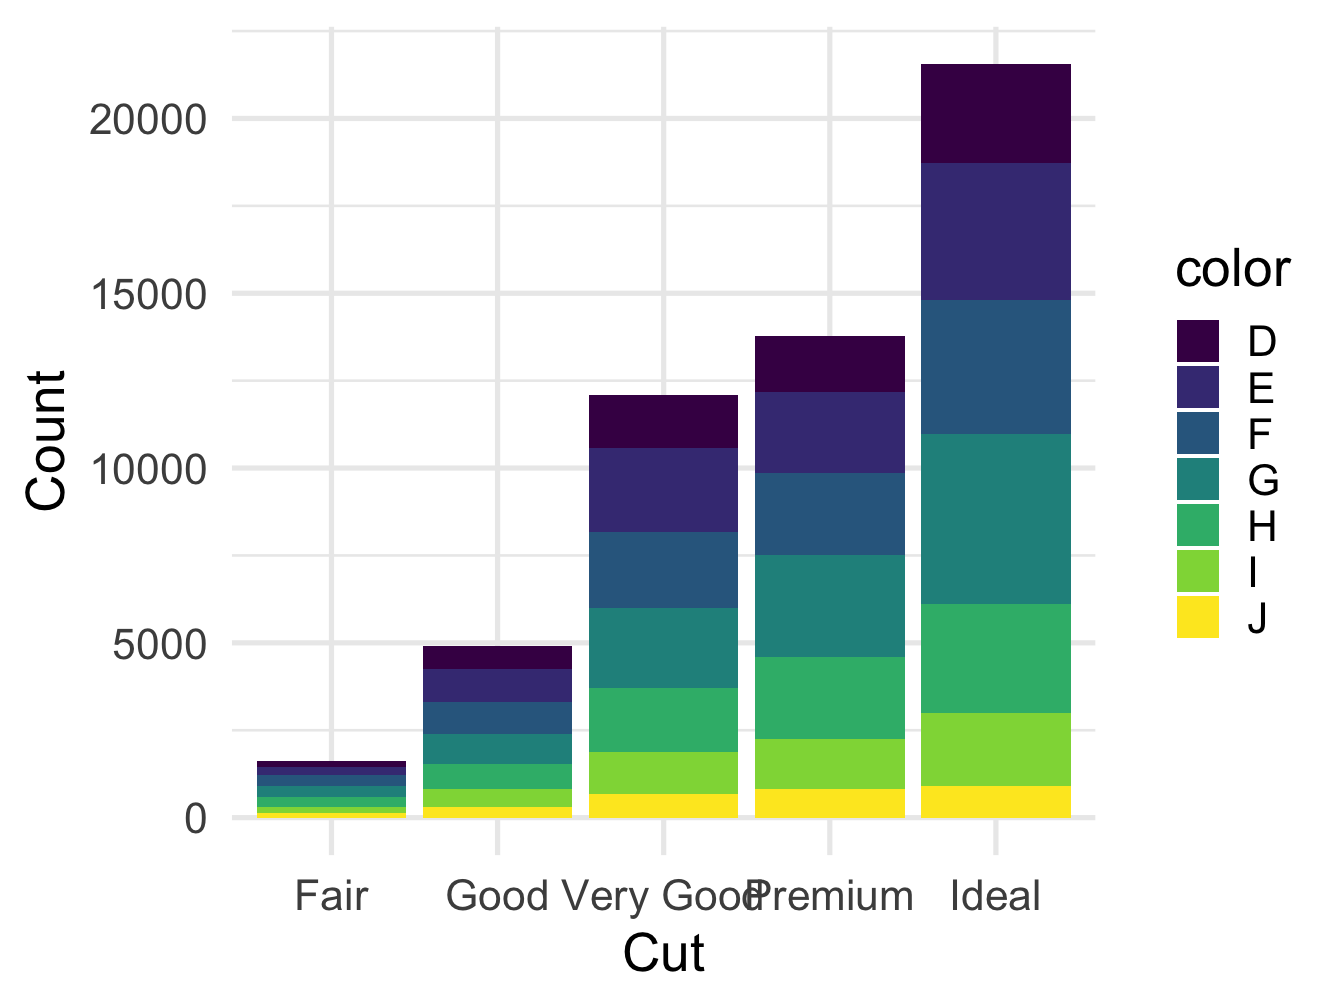
\includegraphics[width=0.8\linewidth]{plotting_r_files/figure-latex/unnamed-chunk-24-1} 

}

\caption{Scatter plot with facets pub quality}\label{fig:unnamed-chunk-24}
\end{figure}

\#\#Correlation plot

\begin{Shaded}
\begin{Highlighting}[]
\NormalTok{diamonds2<-diamonds }\OperatorTok\StringTok{ }\KeywordTok{select}\NormalTok{(depth,table, price,carat)}

\CommentTok{# calulate the correlations}
\NormalTok{c <-}\StringTok{ }\KeywordTok{cor}\NormalTok{(diamonds2, }\DataTypeTok{use=}\StringTok{"complete.obs"}\NormalTok{)}
\end{Highlighting}
\end{Shaded}

\begin{Shaded}
\begin{Highlighting}[]
\KeywordTok{library}\NormalTok{(ggcorrplot)}
\KeywordTok{ggcorrplot}\NormalTok{(c,}\DataTypeTok{lab=}\NormalTok{T, }\DataTypeTok{color=}\KeywordTok{c}\NormalTok{(}\StringTok{"green"}\NormalTok{,}\StringTok{"black"}\NormalTok{,}\StringTok{"orange"}\NormalTok{))}
\end{Highlighting}
\end{Shaded}

\begin{figure}

{\centering 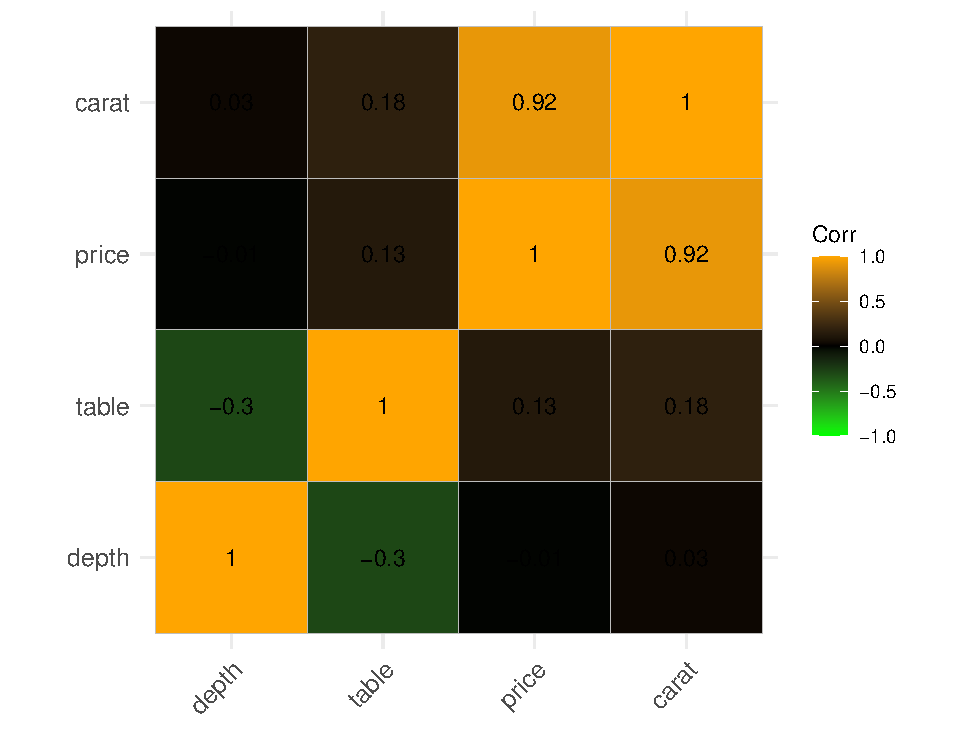
\includegraphics[width=0.8\linewidth]{plotting_r_files/figure-latex/unnamed-chunk-26-1} 

}

\caption{Correlation plot}\label{fig:unnamed-chunk-26}
\end{figure}

  \bibliography{book.bib,packages.bib}

\end{document}
